\documentclass[margin,line]{resume}


\usepackage[utf8]{inputenc}
\usepackage[english,russian]{babel}
\usepackage[T1]{fontenc}
\usepackage{fontawesome}

\usepackage[absolute]{textpos}
\usepackage{enumitem}

\usepackage{graphicx,wrapfig}
\usepackage{url}
\usepackage[colorlinks=true, pdfstartview=FitV, linkcolor=blue,
citecolor=blue, urlcolor=blue]{hyperref}
\pdfcompresslevel=9

\begin{document}
{\sc \large Гришин Антон --- Backend разработчик} \\
\begin{resume}
  \begin{minipage}[t]{0.55\textwidth}
    \section{\mysidestyle Персональная\\Информация}
    Гришин Антон \\
    Москва, Россия \\
    \faLinkedin \space
    \href{https://www.linkedin.com/in/anton-grishin-6966a8362/}{\texttt{anton-grishin}}
    \\
    \faGithub  \space
    \href{https://github.com/alchemmist/}{\texttt{alchemmist}} \\
    \faPaperPlane \space \href{https://t.me/alchemmist}{\texttt{@alchemmist}} \\
    \faPhone \space
    \href{tel:+1234567890}{\color{blue}\texttt{+7(915)067-2638}}  \\
    \faEnvelope \space
    \href{mailto:anton.ingrish@gmail.com}{\color{blue}\texttt{anton.ingrish@gmail.com}}
  \end{minipage}
  \begin{minipage}[H]{0.18\textwidth}
    % 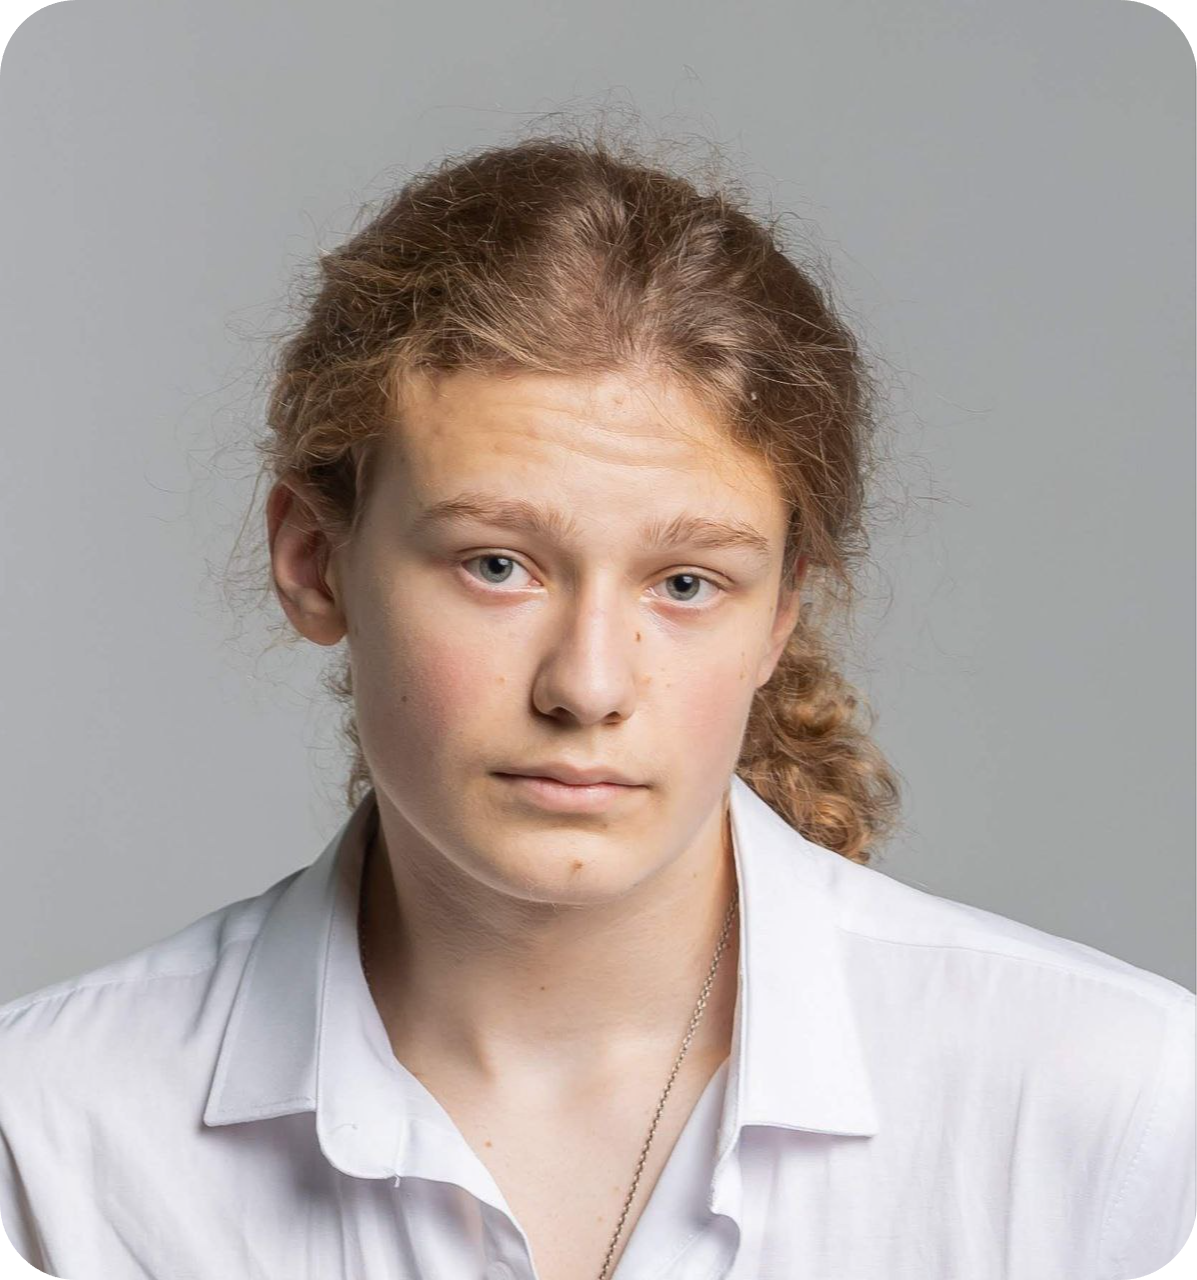
\includegraphics[width=0.45\textwidth]{images/avatar.png}
    % \hspace{5mm}
    \begin{textblock}{7}(10.54, 1.5)
      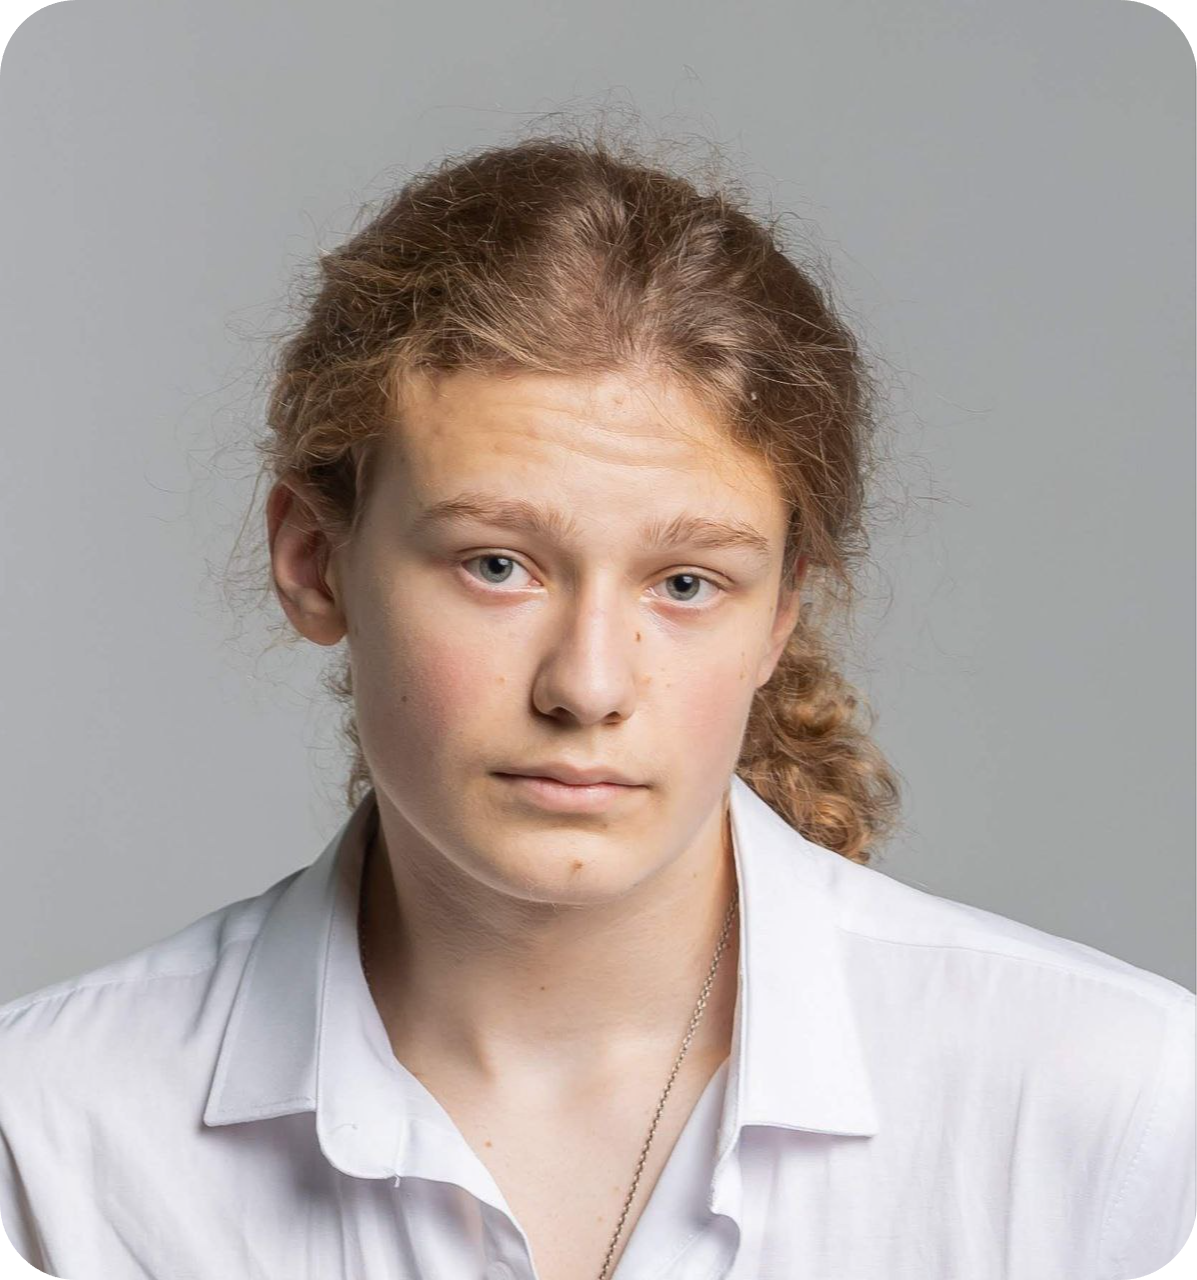
\includegraphics[width=0.27\textwidth]{images/avatar.png}
    \end{textblock}
  \end{minipage}
  \section{\mysidestyle Обо мне}
  В прошлом, я профессиональный воллейболист. Я окончил спортивную
  школу олимпийского резерва, а также инженерный класс Московской школы.

  \section{\mysidestyle Навыки}
  \begin{description}[leftmargin=0pt, itemindent=*]
    \item[Python:] FastAPI, Flask, SqlAlchemy, python-telegram-bot,
      faststream, numpy, pandas.
    \item[Go] FastAPI, Flask, SqlAlchemy, python-telegram-bot,
      faststream, numpy, pandas.
    \item[Databases] Postgres, sqlite, Redis, S3(Yandex Object Storage).
    \item[Message brokers:] RebbitMQ, Kafka, Mosquitto.
    \item[Other techonologies:] SQL, Java, JavaScript, Rust, Latex, Go.
    \item[Scientific softwares] Comsys, Maple, Matlab, Mathematica,
      Scilab, Keysight's VEE and ADS, NI LabVIEW.
    \item[Dev tools:] Neovim, Docker, docker-compose, docker-swarm,
      CI/CD(Github actions, GitLab actions)
    \item[Languages:] Russian, English.
  \end{description}


  \section{\mysidestyle Образование}
  Центральный Университет - Математика и компьютерные науки, 2028

  \section{\mysidestyle Cертификаты}
  \textbf{Яндекс Лицей.} Я экстерном поступил на второй курс Лицея
  Академии Яндекси по Промышленной разработке и окончил его с
  аттистатом с отличием, сдав финальный проект на 100/100 баллов.
  \vspace{-6mm}

  \hfill \textsl{Сентябрь 2022 - Апрель 2023}

  \section{\mysidestyle Достижения}
  \textbf{Прошёл в финал Чемпионата России по спортивному
  программированию,} где наша команда разработала микросервисную
  архитектуру для веб-приложения, агрегирующего спортивные события по
  всей России. (Технологический стек: RabbitMQ (FastStream), FastAPI,
  React, Kafka, OAuth). И разработал алгоритм обработки и проверки
  ежегодных государственных отчетов о спортивных мероприятиях.

  \vspace{-6mm}

  \hfill \textsl{Ноябрь 2024}

      \textbf{Я выиграл научно-практическую конференцию «Наука для жизни»} с проектом умного дома для частных и государственных образовательных учреждений (технологический стек: Redis, Zigbee2MQTT, websockets, Go, Python, Flask, React).
    \vspace{-6mm}

    \hfill \textsl{June 2024}

  \textbf{Участвовал в хакаотне Nuclear IT hack}, где моя команда
    работала над кейсом Росатома по разработке сервиса для определения
    эмоционального тона онлайн-встреч. Я создал
    прототипы и реализовал фронтенд на React, а моя команда
    обучала модель.

    \vspace{-6mm}

    \hfill \textsl{Апрель 2024}

    \section{\mysidestyle Interestings}\vspace{2mm}
    \begin{description}
      \item[Philosophy] Unix, Linux and Windows
      \item[Books:] Unix, Linux and Windows
    \end{description}

    \vfill

    \section{\mysidestyle History}\vspace{2mm}

    \begin{description}

      \item[Measurement Engineer (CNRS)]\small{XLIM \hfill \textsl{June
        2016-Present}}\\
      \item[Lecturer]\small{University of Colorado, Boulder \hfill
        \textsl{January 2016-May 2016}}\\
        ECEN 5014-003, ``Microwave Measurements and Calibration Fundamentals''
        \vspace{2mm}

      \item[Research Associate]\small{University of Colorado at Boulder
        \hfill \textsl{June 2013-May 2016}}\\
        Achievements:
        \begin{list2}
        \item{LabVIEW software for a ``Do-it-yourself'' Large-Signal
          Network Analyzer (LSNA)}
        \item{Time domain measurement setup in Scilab (VTD-SWAP)}
        \item{Outphasing PA characterizations}
        \item{Load-pull in time-domain}
        \end{list2}
        \vspace{2mm}

      \item[Measurement Engineer (CNRS)]\small{XLIM \hfill
        \textsl{December 2007-May 2013}}\\
        Achievements:
        \begin{list2}
        \item{Korrigan European Project activities (RTP
              N$^{\circ}$102.052 funded within the EUROPA framework in the
            CEPA2 priority area - ends early 2009) : GaN HEMTs circuits
            level modeling from european foundries (Thales / QinetiQ) for
          HPA, LNA and Switches}
        \item{Time domain measurement setup (LSNA) development on
          Scilab-TCL/TK (GUI, calibration and measurement automation)}
        \item{Development of HEMTs modeling tools (Scilab)}
        \item{Contractual measurements such as load-pull, linearity,
          high impedance probe in both frequency (VNA) and time domain (LSNA)}
        \end{list2}
        \vspace{2mm}

      \item[Research Associate - Visiting Scholar]\small{University of
        Colorado at Boulder \hfill \textsl{February 2012-July 2012}}\\
        GaN HEMTs based rectifiers characterizations and analysis
        \vspace{2mm}

      \item[Research Engineer (CNRS)]\small{XLIM \hfill \textsl{May
        2005-November 2007}}\\
        Achievements:
        \begin{list2}
        \item{Frequency domain load-pull measurement setup (VNA in
            receiver mode with pulse capabilities) developpemnt with
            Scilab (calibration procedures, measurement automation, data
          processing)}
        \item{Large signal caracterization of transistor (mainly
            european GaN in the framework of Korrigan}
          \item{Korrigan WP3.3 workpackage leader in Korrigan.
              Developpement of a internet database (Php / mySQL) to let
            partners share data and informations}
          \item{GaN HEMTs ``spice-like'' nonlinear models}
          \end{list2}
          \vspace{2mm}

        \item[Research Engineer]\small{NMDG Engineering bvba \hfill
          \textsl{November 2004-February 2005}}\\
          Implementation of the High Impedance Probe module
          (calibration and measurements) in the commercial LSNA
          Software (based on Mathematica)

          \vspace{2mm}

        \item[Postdoctoral scientist]\small{CNES (French Space Agency)
          \hfill \textsl{October 2003-September 2004}}\\
          Development of characterization tools interfaces within the
          free open-source scientific package Scilab

          \vspace{2mm}

        \item[Postdoctoral scientist]\small{CNES (French Space Agency)
          \hfill \textsl{October 2002-September 2003}}\\
          Achievements:
          \begin{list2}
          \item{Large Signal Network Analysis (LSNA) characterizations
            in time-domain}
          \item{Development of a new LSNA module in order to
              investigate time domain waveforms at internal nodes of
              MMICs with high impedance probes (HIP) to validate circuits
            designs and to analyze nonlinear parametric stability}
          \item{Large Signal Network Analysis (LSNA) characterizations
            in time-domain}
          \end{list2}
          \vspace{2mm}

        \item[Researcher]\small{IRCOM / University of Limoges \hfill
          \textsl{October 1998-September 2002}}\\
          Achievements:
          \begin{list2}
          \item{Development of the RF time-domain envelope measurement
            setup (hardware and software)}
          \item{Development of the calibration procedure of the
            time-domain envelope measurement setup}
          \item{Power amplifiers characterizations : Load-pull, IM3, NPR}
          \item{Behavioral modeling of nonlinear devices with memory
            effects for system level}
          \item{Development of a dynamic complex gain model with
            neural networks}
          \end{list2}
          \vspace{2mm}

        \item[Lecturer]\small{University of Limoges \hfill
          \textsl{October 1998-September 2002}}\\
          RF devices, analog/digital communication systems, signal
          processing, propagation waves...
          \vspace{2mm}

        \item[Postgraduate student]\small{IRCOM / University of Limoges
          \hfill \textsl{February 1998-July 1998}}\\
          Circuits level simulations of IM3 and NPR in order to
          optimize the trade-off between linearity and efficiency

      \end{description}

    \end{resume}
    \end{document}
